%----------------------------------------------------------------------------------------
%	PACKAGES AND OTHER DOCUMENT CONFIGURATIONS
%----------------------------------------------------------------------------------------

\documentclass[11pt,a4paper]{article}

\usepackage[utf8]{inputenc}
\usepackage[dutch]{babel}
\usepackage{amsmath}
\usepackage{amsfonts}
\usepackage{amssymb}
\usepackage[left=2cm,right=2cm,top=2cm,bottom=2cm]{geometry}
\usepackage{graphicx}
\usepackage{float}
\graphicspath{{figures/}}
\usepackage{todonotes}
\usepackage{url}

%----------------------------------------------------------------------------------------
%	CONFIGURATION OF CODE LISTINGS
%----------------------------------------------------------------------------------------

\usepackage{listings}
\usepackage{color}
 
\definecolor{codegreen}{rgb}{0,0.6,0}
\definecolor{codegray}{rgb}{0.5,0.5,0.5}
\definecolor{codepurple}{rgb}{0.58,0,0.82}
\definecolor{backcolour}{rgb}{0.95,0.95,0.92}
 
\lstdefinestyle{mystyle}{
    backgroundcolor=\color{backcolour},   
    commentstyle=\color{codegreen},
    keywordstyle=\color{magenta},
    numberstyle=\tiny\color{codegray},
    stringstyle=\color{codepurple},
    basicstyle=\footnotesize,
    breakatwhitespace=false,         
    breaklines=true,                 
    captionpos=b,                    
    keepspaces=true,                 
    numbers=left,                    
    numbersep=5pt,                  
    showspaces=false,                
    showstringspaces=false,
    showtabs=false,                  
    tabsize=2
}
 
\lstset{style=mystyle}

\begin{document}

\begin{titlepage}

\newcommand{\HRule}{\rule{\linewidth}{0.5mm}} % Defines a new command for the horizontal lines, change thickness here

\center % Center everything on the page
 
%----------------------------------------------------------------------------------------
%	HEADING SECTIONS
%----------------------------------------------------------------------------------------

\textsc{\textsc{\LARGE KU Leuven}}\\[1.5cm] % Name of your university/college
\textsc{\Large Modellering \& Simulatie}\\[0.5cm] % Major heading such as course name
\textsc{\large Verslag practicum 1}\\[0.5cm] % Minor heading such as course title

%----------------------------------------------------------------------------------------
%	TITLE SECTION
%----------------------------------------------------------------------------------------

\HRule \\[0.4cm]
{ \huge \bfseries Lagerangbenadering}\\[0.4cm] % Title of your document
\HRule \\[1.5cm]
 
%----------------------------------------------------------------------------------------
%	AUTHOR SECTION
%----------------------------------------------------------------------------------------

\begin{minipage}{0.4\textwidth}
\begin{flushleft} \large
\emph{Auteur:}\\
Ward \textsc{Schodts} % Your name
\end{flushleft}
\end{minipage}
~
\begin{minipage}{0.4\textwidth}
\begin{flushright} \large
\emph{Begeleiders:} \\
Prof. Dr. Ir. Ronald \textsc{Cools} \\ % Supervisor's Name
Prof. Dr. Ir. Wim \textsc{Michiels} \\ % Supervisor's Name
Prof. Dr. Ir. Dirk \textsc{Nuyens} \\ % Supervisor's Name
Dr. Ir. Nick \textsc{Vannieuwenhoven} \\ % Supervisor's Name
\end{flushright}
\end{minipage}\\[4cm]

% If you don't want a supervisor, uncomment the two lines below and remove the section above
%\Large \emph{Author:}\\
%John \textsc{Smith}\\[3cm] % Your name

%----------------------------------------------------------------------------------------
%	DATE SECTION
%----------------------------------------------------------------------------------------

{\large \today}\\[3cm] % Date, change the \today to a set date if you want to be precise

%----------------------------------------------------------------------------------------
%	LOGO SECTION
%----------------------------------------------------------------------------------------


\includegraphics[scale=0.15]{sedes}\\[1cm] % Include a department/university logo - this will require the graphicx package
 
%----------------------------------------------------------------------------------------

\vfill % Fill the rest of the page with whitespace

\end{titlepage}

\section*{Opdracht 1}

\lstinputlisting[language=Matlab, caption=Opdracht 1, firstline=1, lastline=5]{../opdrachten.m}

\section*{Opdracht 2}

\lstinputlisting[language=Matlab, caption=Opdracht 2]{../r0381767_approximationError.m}

\section*{Opdracht 3}
\todo{rank nog wegdoen}
\lstinputlisting[language=Matlab, caption=Opdracht 3]{../r0381767_predictedRatings.m}

\section*{Opdracht 4}

\begin{figure}[H]
\centering
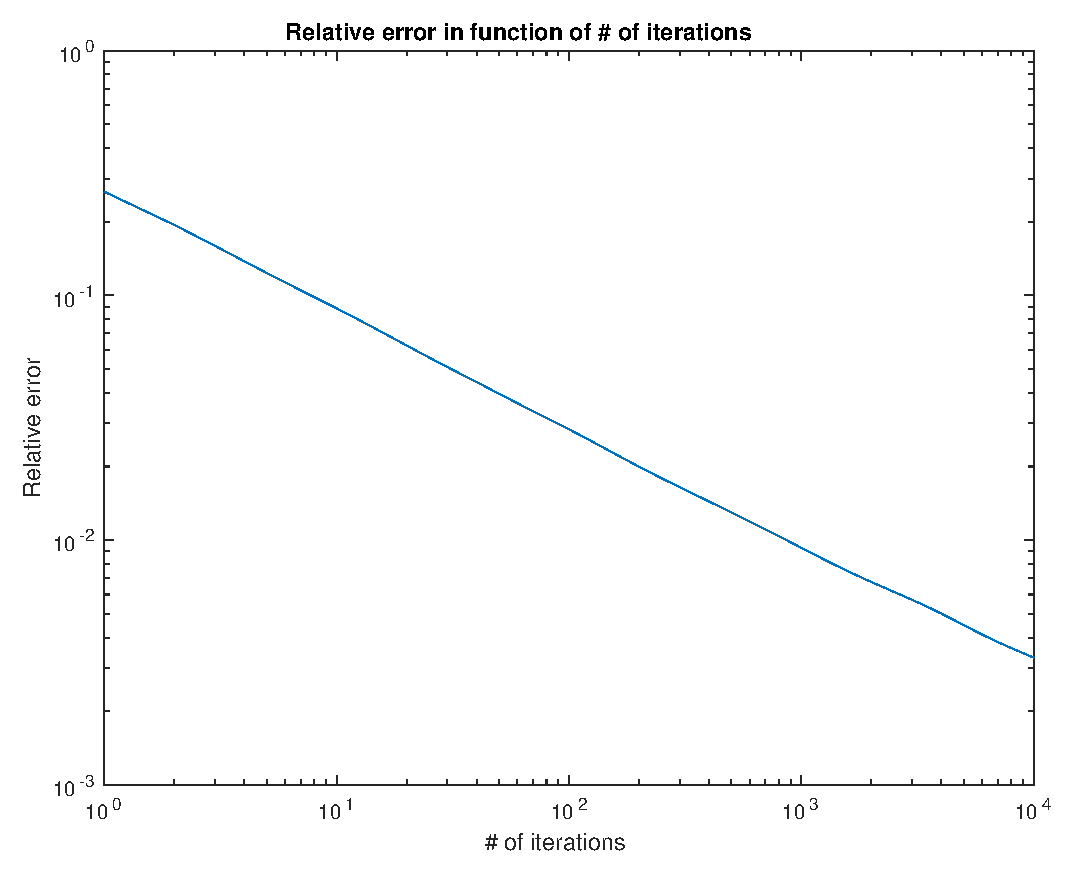
\includegraphics[scale=0.55]{opdracht4}
\caption{Opdracht 4}
\end{figure}

Een rechte op een loglog plot heeft een vergelijking van volgende vorm:

\begin{equation}
\log_{10}(y) = m\log_{10}x + b 
\end{equation}
\textit{y} is de benaderningsfout.\\
\textit{x} is de iteratie waarin dat fout \textit{y} is.\\
\textit{b} is het snijpunt van de rechte met de y-as \\
\textit{m} is de richtingscoëfficient en hier ook convergentiefactor. Aangezien het een dalende rechte is moet m negatief zijn.\\
We bepalen nu de convergentie-orde met behulp van volgende formule:
$$\lim_{k\rightarrow\infty} \frac{|e_{k+1} - L|}{|e_k - L|} = \mu$$
Hier is \textit{L} het getal waarnaar geconvergeerd wordt, in dit geval dus 0, we krijgen:
\begin{equation}
\lim_{k\rightarrow\infty} \frac{|e_{k+1}|}{|e_k|} = \mu
\end{equation}
$e_k$ en $e_{k+1}$ stellen dus respectievelijk de k-de en k+1-ste fout voor. Deze fouten kunnen we halen uit vergelijking (1):
$$\text{fout k} = y = x^m + 10^b$$

Indien we dit invullen in vergelijking (2) krijgen we:

$$\lim_{k\rightarrow\infty} \frac{|(k+1)^m + 10^b|}{|k^m + 10^b|} = 1$$


Aangezien $\mu=1$ wordt voor $k\rightarrow \infty$ kunnen we spreken over \textbf{sublineare convergentie orde}\footnote{\url{https://en.wikipedia.org/wiki/Rate_of_convergence}}. 

\lstinputlisting[language=Matlab, caption=Opdracht 4, firstline=6, lastline=13]{../opdrachten.m}

\section*{Opdracht 5}
De kleinste rang waarvoor de benaderingsfout kleiner is als $10^{-13}$ is 26.
Dit valt af te lezen van de figuur alsook in de vector \texttt{Error} in onderstaande code waarbij het 26ste element 0.000000000000003 is, terwijl het 25ste nog 0.000000000005736 is en dus groter als $10^{-13}$.
\begin{figure}[H]
\centering
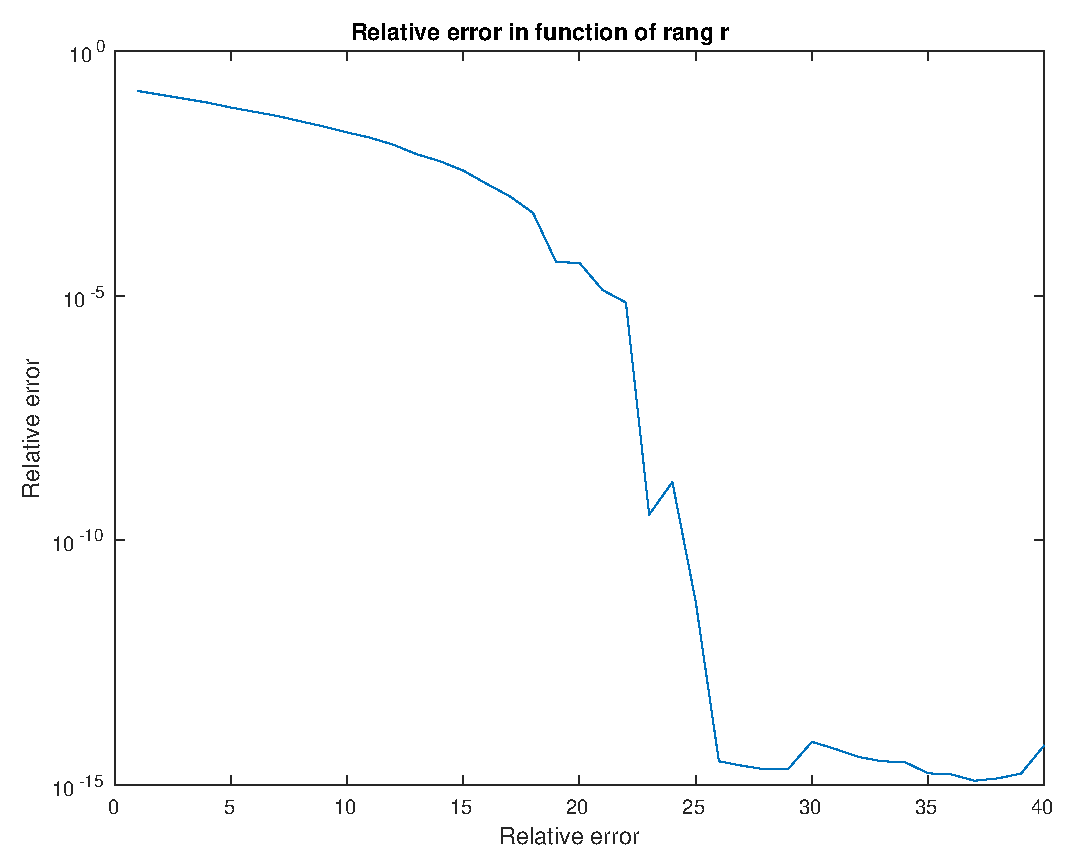
\includegraphics[scale=0.55]{opdracht5}
\caption{All approximation errors}
\end{figure}

\lstinputlisting[language=Matlab, caption=Opdracht 5]{../r0381767_plotAllApproximationErrors.m}
\lstinputlisting[language=Matlab, caption=Hulproutine voor opdracht 5]{../r0381767_predictedError.m}

\section*{Opdracht 6}

\begin{figure}[H]
\centering
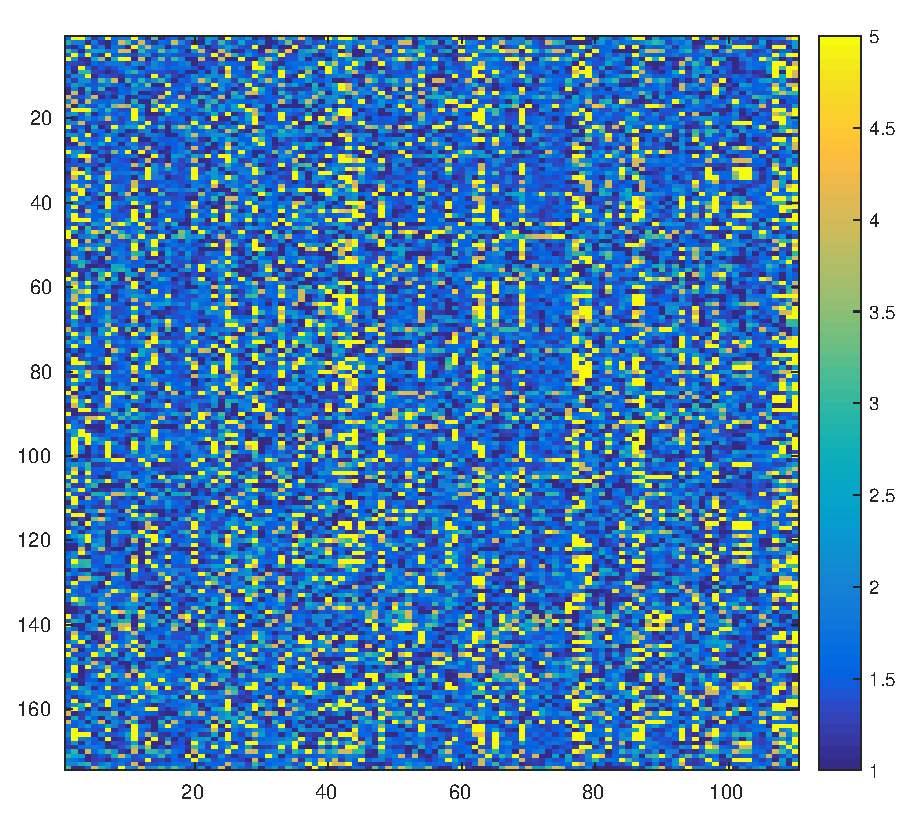
\includegraphics[scale=0.55]{opdracht6}
\caption{Predicted26}
\end{figure}

\lstinputlisting[language=Matlab, caption=Opdracht 4, firstline=19, lastline=24]{../opdrachten.m}

\section*{Opdracht 7}

\lstinputlisting[language=Matlab, caption=Opdracht 7]{../r0381767_similarBooks.m}

\section*{Opdracht 8}
Onderstaande lijst geeft boeken die bij elkaar zouden moeten horen voor boek 1, 21 en 101.
De resultaten zijn zeer realistisch aangezien er telkens de andere boeken teruggeven worden van dezelfde reeks.\\
\textbf{Boek 1:}
\begin{enumerate}
\item Harry Potter and the Sorcerer's Stone
\item Harry Potter and the Chamber of Secrets
\item Harry Potter And The Goblet Of Fire (Book 4)
\item Harry Potter And The Prisoner Of Azkaban
\item Harry Potter and the Order of the Phoenix (Book 5)
\item Harry Potter and the Half-Blood Prince
\end{enumerate}
\textbf{Boek 21:}
\begin{enumerate}
\item A Game of Thrones: A Song of Ice and Fire: Book One
\item A Clash of Kings: A Song of Ice and Fire: Book Two (Game of Thrones)
\item A Feast for Crows (A Song of Ice and Fire)
\end{enumerate}
\textbf{Boek 101:}
\begin{enumerate}
\item The Arrangement 2
\item The Arrangement 3 (Volume 3)
\item The Arrangement 11: The Ferro Family  (Volume 11)
\item The Arrangement 4 (Volume 4)
\item The Arrangement Vol. 8: The Ferro Family (Volume 8)
\item The Arrangement 13 (The Ferro Family) (Volume 13)
\item The Arrangement 5 (Volume 5)
\item The Arrangement 12 (The Ferro Family) (Volume 12)
\item The Arrangement 14 (The Ferro Family) (Volume 14)
\item The Arrangement 9: The Ferro Family (Volume 9)
\end{enumerate}

\lstinputlisting[language=Matlab, caption=Opdracht 8, firstline=27, lastline=31]{../opdrachten.m}


\section*{Opdracht 9}
Figuur 4 toont inderdaad aan dat de singuliere waarden met volgnummer strikt groter dan 26 niet van de grootte-orde $10^{-13}$ zijn:
\begin{figure}[H]
\centering
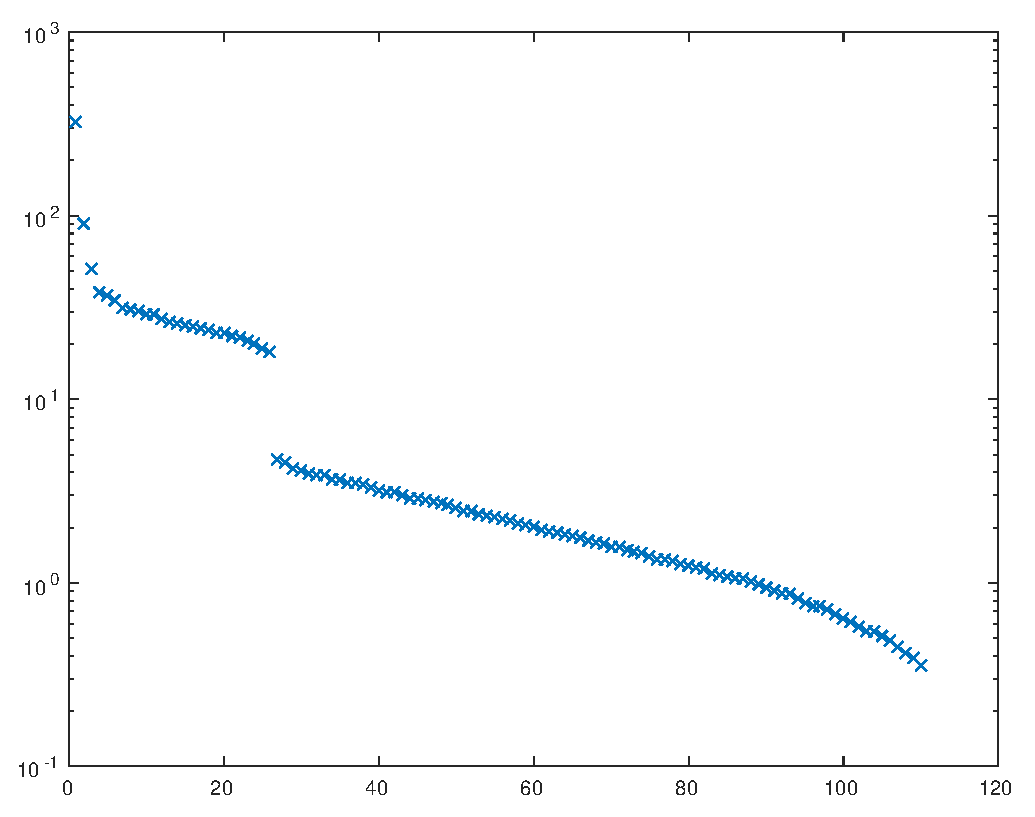
\includegraphics[scale=0.55]{opdracht9a}
\caption{Singuliere waarden na afronding}
\end{figure}

Dit is te verklaren door de laatste stap het iteratief algoritme dat geïmplementeerd is in \\opdracht 3:
$$A \leftarrow max\{1,min\{5,A_{\kappa}\}\}$$
Deze stap zorgt er voor dat alle waarden binnen de schaal van 1 tot 5 liggen. Waarden kleiner dan 1 en groter dan 5 worden respectievelijk vergroot en verkleind. Hoewel dit niet uitmaakt voor de uiteindelijke benaderingsmatrix die wordt berekend door het algoritme, heeft dit wel invloed op de singuliere waarden. Om dit aan te tonen kan men dezelfde plot nemen van het algoritme voordat de afrondingen gebeurd zijn. Dit is te zien op lijn 23 en 24 van listing 3. 
\begin{figure}[H]
\centering
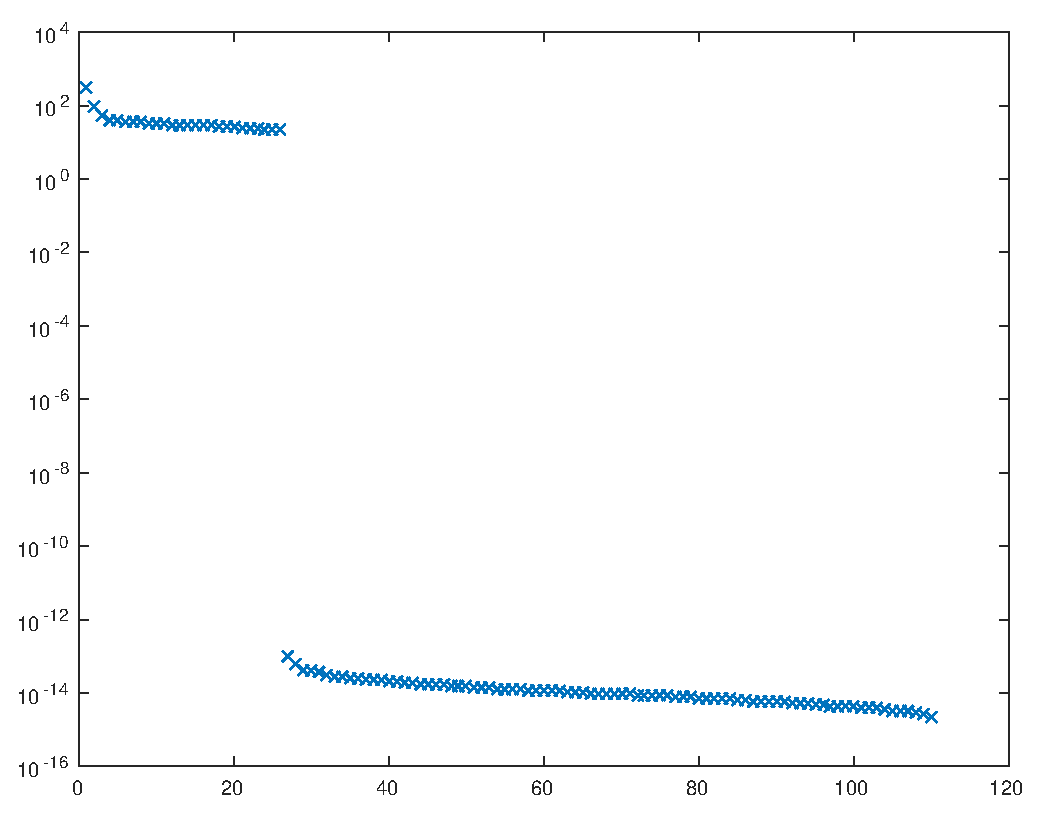
\includegraphics[scale=0.55]{opdracht9b}
\caption{Singuliere waarden zonder afronding}
\end{figure}
Inderdaad, in figuur 5 hebben de singuliere waarden met volgnummers strikt groter dan 26 nu wel een grootte-orde van $10^{-13}$.\\
\\
Dit fenomeen kan ook nog iets formeler verklaard worden. Singuliere waarden zijn de vierkantswortels van niet negatieve eigenwaarden. We weten ook dat het aantal niet nul eigenwaarden (van een matrix) kleiner dan of gelijk is, als de rang van die matrix.
Als er dus een benadering wordt gemaakt van rang \textit{r} door het algoritme in opdracht 3, dan zouden er dus telkens maar maximaal \textit{r} singuliere waarden mogen bestaan. De singuliere waarden die van grootte-orde $10^{-13}$ zijn, mogen we dus verwaarlozen.
\\
\\
Door de afronding die gebeurd in de laatste stap van het algoritme veranderd de rang van de berekende matrix. Als we de rang berekenen voor de afronding (in lijn 22 bij listing 3) dan zien we dat die overeen komt met de parameter \textit{r=26}. De rang na afronding komt overeen met 110. Hierdoor is er geen enkele singuliere waarde die in buurt komt van grootte-orde $10^{-13}$.

\lstinputlisting[language=Matlab, caption=Opdracht 9, firstline=33, lastline=36]{../opdrachten.m}

\section*{Opdracht 10}

\lstinputlisting[language=Matlab, caption=Opdracht 10]{../r0381767_correlationMatrix.m}

\section*{Opdracht 11}

\begin{figure}[H]
\centering
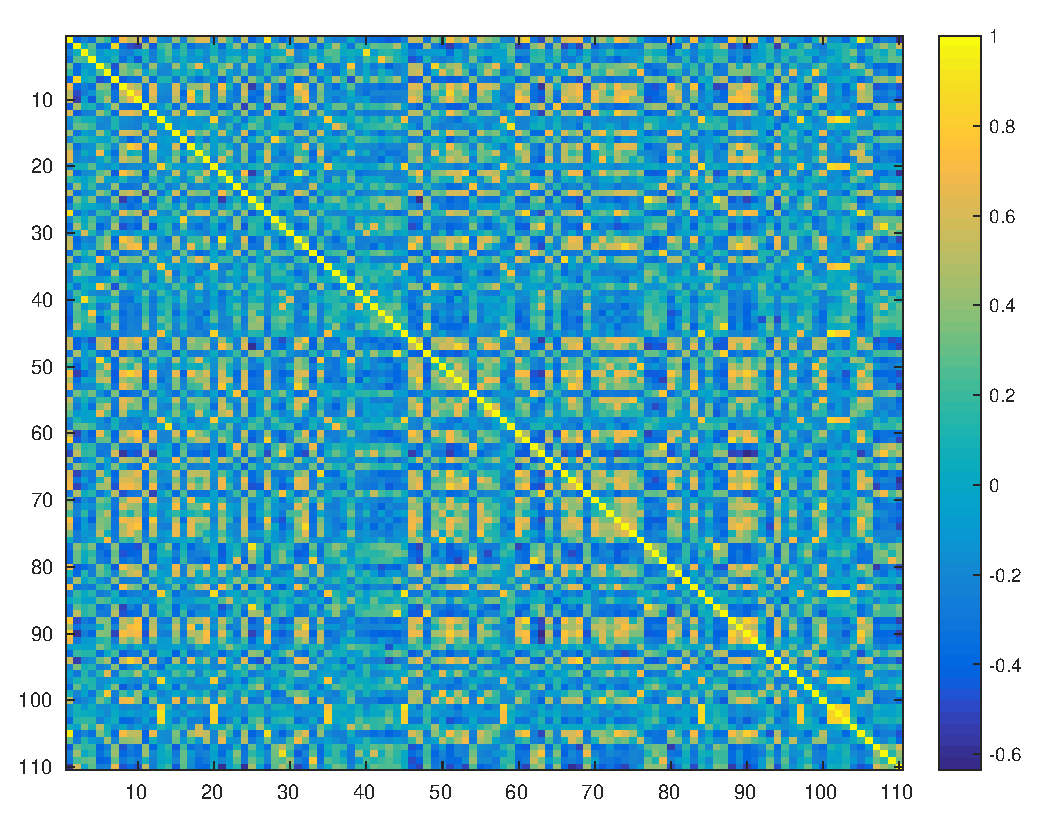
\includegraphics[scale=0.55]{opdracht11}
\caption{Correlatiematrix van Predicted26}
\end{figure}

\lstinputlisting[language=Matlab, caption=Opdracht 9, firstline=38, lastline=43]{../opdrachten.m}

\section*{Opdracht 12}

\lstinputlisting[language=Matlab, caption=Opdracht 12]{../r0381767_buildCliques.m}

\section*{Opdracht 13}

\begin{figure}[H]
\centering
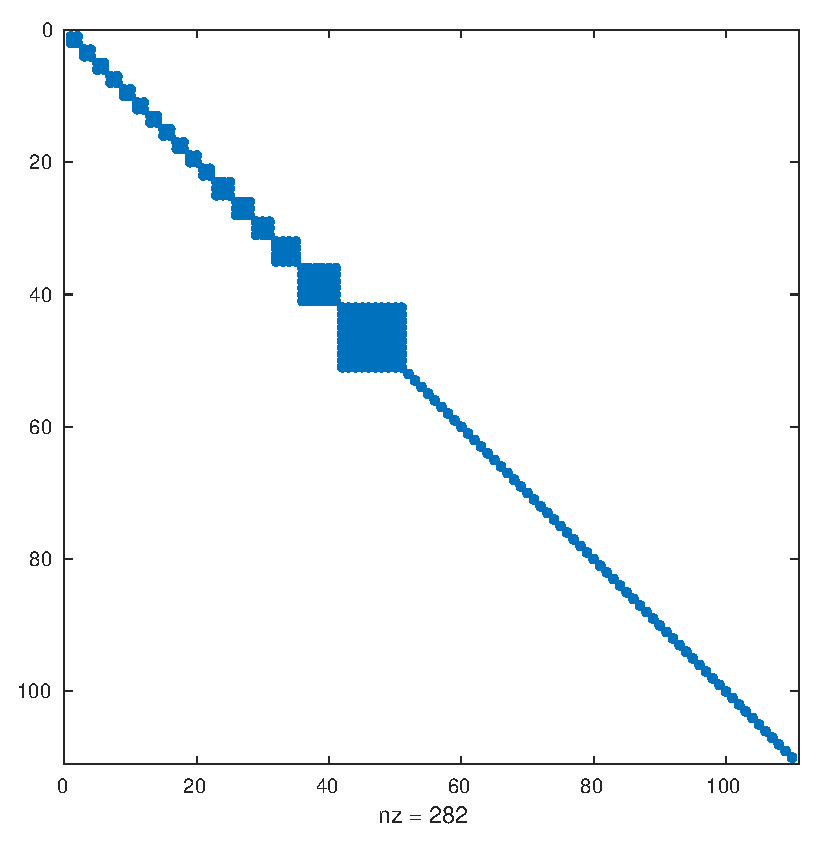
\includegraphics[scale=0.65]{opdracht13a}
\caption{Opdracht 13}
\end{figure}

\begin{figure}[H]
\centering
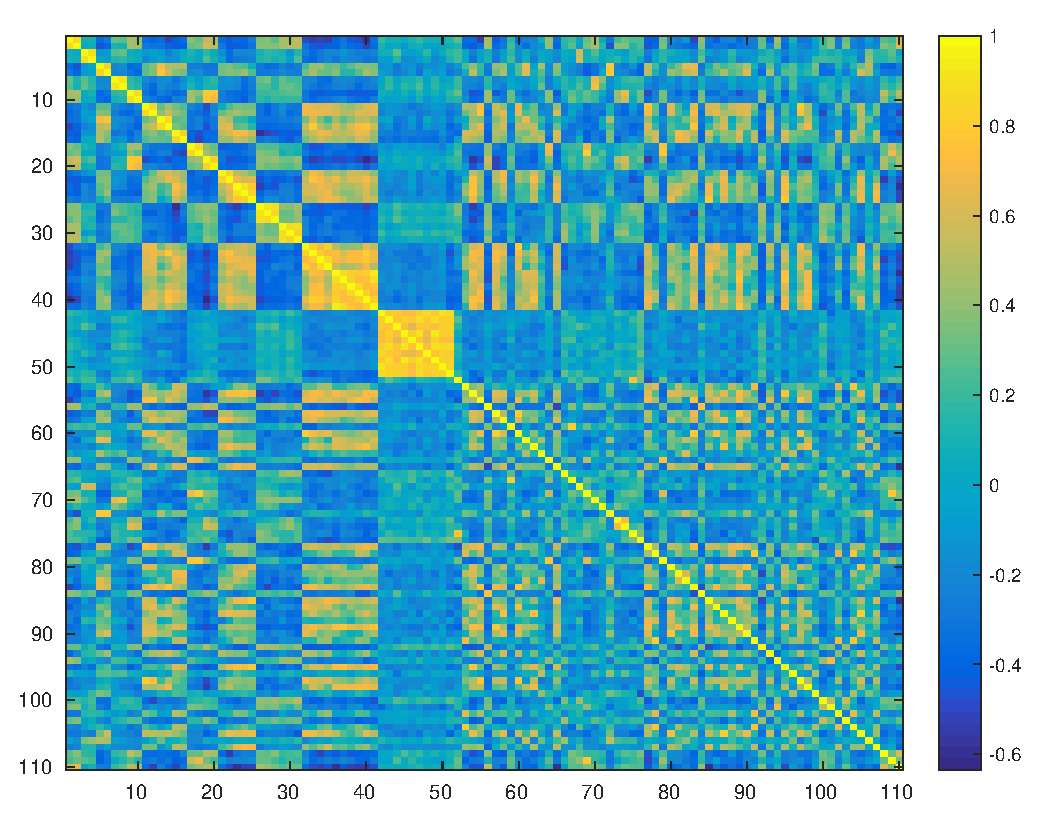
\includegraphics[scale=0.55]{opdracht13b}
\caption{Opdracht 13}
\end{figure}

\lstinputlisting[language=Matlab, caption=Opdracht 13, firstline=45, lastline=56]{../opdrachten.m}

\section*{Opdracht 14}

\lstinputlisting[language=Matlab, caption=Opdracht 14]{../r0381767_cluster.m}
\lstinputlisting[language=Matlab, caption=Hulproutine opdracht 14]{../r0381767_findClusterAt.m}

\section*{Opdracht 15}

\textbf{Cluster 1:}
\begin{enumerate}
\item A Game of Thrones: A Song of Ice and Fire: Book One
\item A Clash of Kings: A Song of Ice and Fire: Book Two (Game of Thrones)
\item A Feast for Crows (A Song of Ice and Fire)
\end{enumerate}
\textbf{Cluster 2:}
\begin{enumerate}
\item This Man
\item Beneath This Man (This Man Trilogy)
\item This Man Confessed (This Man Trilogy)
\end{enumerate}
\textbf{Cluster 3:}
\begin{enumerate}
\item Fueled (The Driven Trilogy)
\item Crashed (The Driven Trilogy)
\item Driven ((The Driven Trilogy))
\end{enumerate}
\textbf{Cluster 4:}
\begin{enumerate}
\item Slaughterhouse-Five (or The Children's Crusade: A Duty Dance with Death)
\item Nineteen Eighty Four (Penguin Modern Classics)
\item The Girl with the Dragon Tattoo
\item Memoirs of a Geisha
\end{enumerate}
\textbf{Cluster 5:}
\begin{enumerate}
\item Harry Potter and the Sorcerer's Stone
\item Harry Potter and the Chamber of Secrets
\item Harry Potter And The Goblet Of Fire (Book 4)
\item Harry Potter And The Prisoner Of Azkaban
\item Harry Potter and the Order of the Phoenix (Book 5)
\item Harry Potter and the Half-Blood Prince
\end{enumerate}
\textbf{Cluster 6:}
\begin{enumerate}
\item The Arrangement 2
\item The Arrangement 3 (Volume 3)
\item The Arrangement 11: The Ferro Family  (Volume 11)
\item The Arrangement 4 (Volume 4)
\item The Arrangement Vol. 8: The Ferro Family (Volume 8)
\item The Arrangement 13 (The Ferro Family) (Volume 13)
\item The Arrangement 5 (Volume 5)
\item The Arrangement 12 (The Ferro Family) (Volume 12)
\item The Arrangement 14 (The Ferro Family) (Volume 14)
\item The Arrangement 9: The Ferro Family (Volume 9)
\end{enumerate}
Buiten cluster 4 zijn de resultaten op het eerste zicht zeer goed te vertrouwen. Het zijn telkens boeken van dezelfde reeks. 
Cluster 4 echter niet. Maar dit betekent niet dat het niet te verklaren is dat ze bij elkaar horen. 
Ze zijn niet van hetzelfde genre, noch van dezelfde auteur. Als je in google zoekt op \textit{"girl with the dragon tattoo"+"memoirs of a geisha"+ "nineteen eighty four"+ "slaughterhouse-five"} dan wordt het verband duidelijk. 
Deze vier boeken komen vaak samen voor op reading lists. Daarenboven zijn ze ook alle vier verfilmd.
Dit gaat waarschijnlijk de oorzaak zijn dat er een cluster is gevormd.

\lstinputlisting[language=Matlab, caption=Opdracht 15, firstline=58, lastline=69]{../opdrachten.m}

\section*{Opdracht 16}

\begin{figure}[H]
\centering
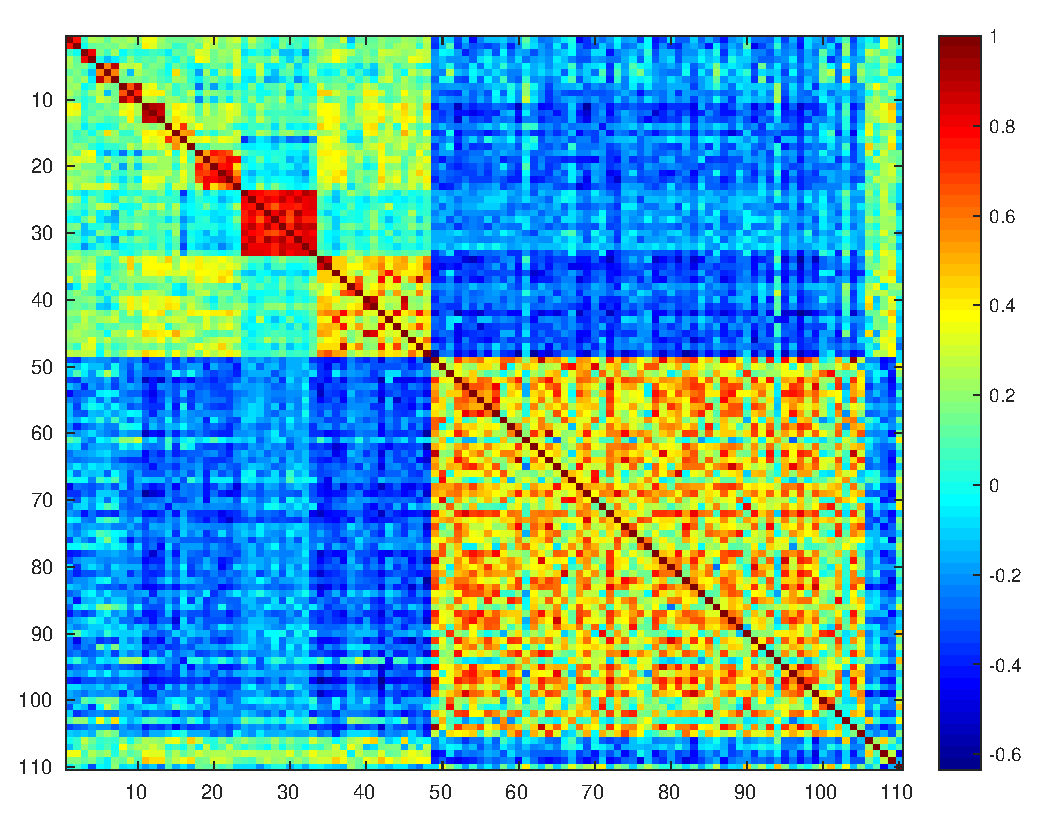
\includegraphics[scale=0.55]{opdracht16}
\caption{Opdracht 16}
\end{figure}
De bijzondere structuur van figuur 9 is te verklaren doordat de correlatiematrix een symmetrisch matrix is. Daarna gaat het commando \texttt{symamd} er nog voor zorgen dat er
\lstinputlisting[language=Matlab, caption=Opdracht 15, firstline=71, lastline=79]{../opdrachten.m}

\section*{Opdracht 17}

We moeten dus bewijzen dat:
$$ rang(C) = rang\left(\frac{1}{m-1}((A-1\mu^T)\Sigma^{-1})^T((A-1\mu^T)\Sigma^{-1})\right) \leq r + 1$$
De rang wordt niet beïnvloed door te vermenigvuldigen met een scalar:
$$ rang(C) = rang\left(((A-1\mu^T)\Sigma^{-1})^T((A-1\mu^T)\Sigma^{-1})\right) \leq r + 1$$
We gebruiken nu volgende eigenschap van matrices:
\begin{equation}
rang(A^TA) = rang(AA^T) = rang(A) = rang(A^T)
\end{equation}
Dan bekomen we:
$$ rang(C) = rang\left((A-1\mu^T)\Sigma^{-1}\right) \leq r + 1$$
$\Sigma$ is een diagonaalmatrix van rang n, dan kunnen we volgende eigenschap gebruiken:
\\
\\
Indien A een $m\times n$ matrix is en B een $n\times k$ matrix van rang n dan geldt:
\begin{equation}
rang(AB) = rang(A)
\end{equation}
Nu bekomen we:

$$ rang(C) = rang\left(A-1\mu^T\right) \leq r + 1$$
\\
We kunnen nu de eigenschap van subaddiviteit toepassen:
\begin{equation}
rang(A+B) \leq rang(A) + rang(B)
\end{equation} 
Dan bekomen we uiteindelijk:
$$  rang(C) = rang\left(A+(-1\mu^T)\right) = rang(A) + rang(-1\mu^T) \leq r + 1$$
De vorige eigenschap in (4) kunnen we nu ook gebruiken om de rang van $1\mu^T$ te berekenen. Aangezien $1$ en $\mu$ 1-dimensionaal zijn is hun rang ook maximaal 1. De rang van was al gekend namelijk \textit{r}. Hiermee is het gevraagde aangetoond.

\section*{Opdracht 18}

We moeten aantonen dat het matrixproduct $K = H^2 = H\cdot H$ enkel van nul verschilt indien er een pad bestaat van hoogstens lengte 2.
\\
\\
In de incidentiematrix H staat er enkel een getal verschillend van 1 als er een rechtstreeks pad is tussen twee knopen (hier boeken).
\\
\\
We bewijzen nu in twee richtingen:\\
\underline{$K = H^2 = H\cdot H$ verschilt van nul $\Rightarrow$ er bestaat een pad van hoogstens lengte 2:}
\\
\\
f
\\
\\
\underline{Er bestaat een pad van hoogstens lengte 2 $\Rightarrow$ $K = H^2 = H\cdot H$ verschilt van nul:}
\\
\\
Het matrixproduct is gedefineerd als:
$$(AB)_{ij} = \sum_{k=1}^mA_{ik}B_{kj}$$
In de matrix K kan dus enkel een nul verschijnen indien de elementen in een rij i van H paarsgewijs vermenigvuldigd met de elementen uit een kolom j van H allemaal 0 zijn. We veronderstelden net het omgekeerde namelijk $(AB)_{ij} \neq 0$. Dit betekent dat er in H een rij en kolom waarbij geld dat er paden van lengte 2 zijn.

\section{•}
\end{document}